\subsection{Ellipsoids}
\noindent
Ellipsoids look like ellipses that have been rotated and extruded about their axis.
They are radially symmetric about this axis.
They have the general form 
\begin{equation*}
	d = \frac{x^2}{a^2} + \frac{y^2}{b^2} + \frac{z^2}{c^2}	
\end{equation*}
Note that the only difference in the equation between an ellipsoid and hyperboloid is the signs are all positive.

\begin{figure}[H]
	\centering
	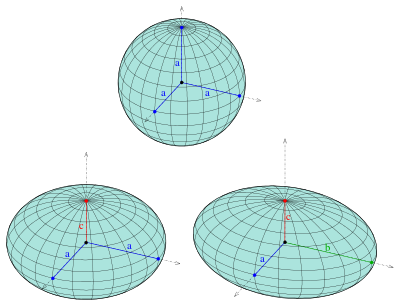
\includegraphics[width=0.66\textwidth]{./Images/differentialMultivariableCalculus/ellipsoids.png}
	\caption{Ellipsoids}
\end{figure}